\section{The physics behind X-ray diffraction}

Max von Laue discovered the phenomena of diffraction of X-rays by crystals, for which he was awarded the Nobel Prize in Physics in 1914. Laue viewed the three-dimensional periodic arrangement of atoms in a crystal as a 3D diffraction grating, and thereby derived a condition which needs to be satisfied for the diffraction of X-rays to take place.

Sir William Henry Bragg and William Lawrence Bragg furthered the physics of X-ray diffraction. Lawrence Bragg, in contrast to Laue's work, viewed the layers (planes) of atoms in the crystal lattice as reflecting surfaces, and X-ray beams reflecting off consecutive planes would interfere constructively if a certain condition was satisfied. This theory is not true in the physical sense -- planes of atoms do not reflect X-rays as such -- but it is correct in the geometrical sense, and we can arrive at Bragg's Law if we start from Laue's condition. The Braggs were jointly awarded the Nobel prize in Physics in 1915 for their work in X-ray crystallography.

\subsection{Bragg's Analysis}
	
	\begin{figure}
	\centering
	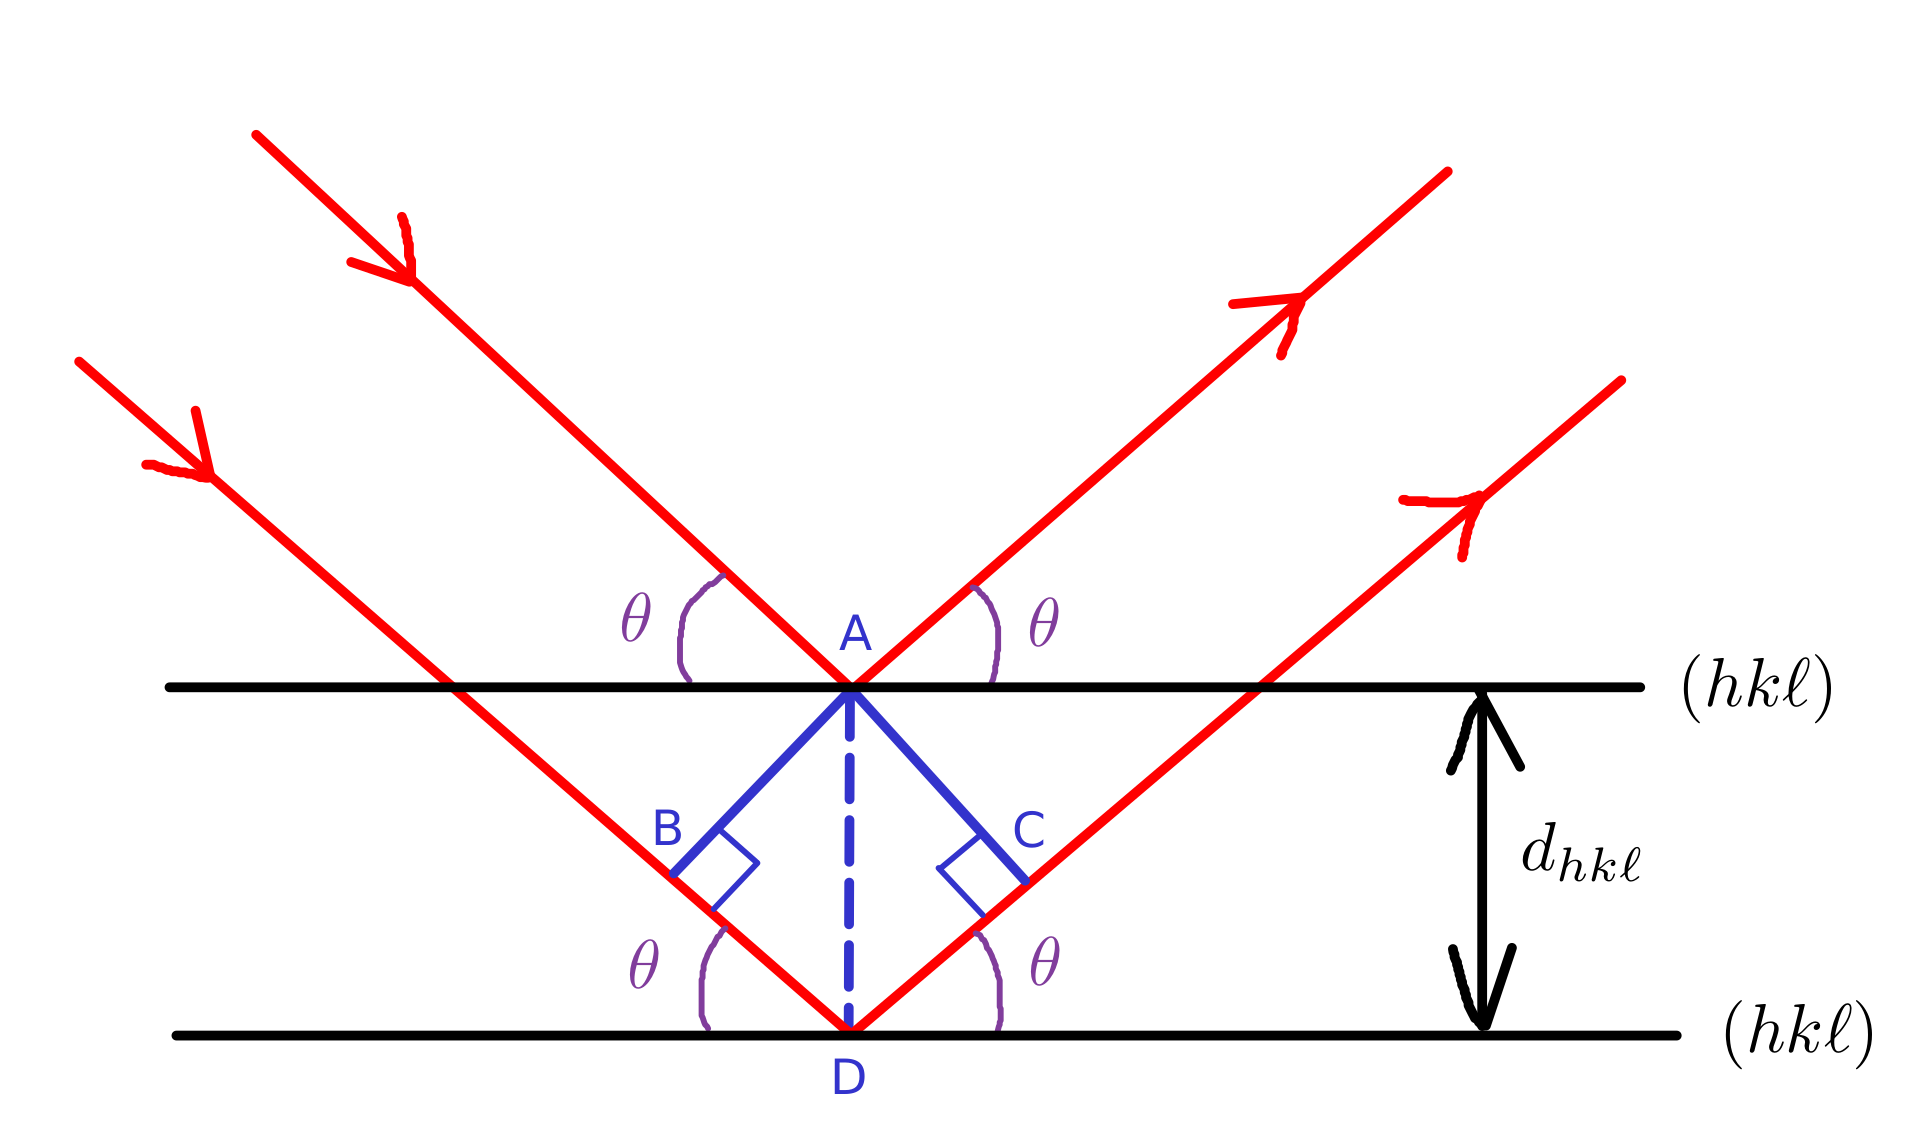
\includegraphics[scale=0.15]{bragg_law.png}
	\caption{\label{fig:bragg_law}X-ray beam is incident on a set of planes with Miller indices $(hk\ell),$ as shown. We draw perpendiculars $\mathrm{AB}$ and $\mathrm{AC}$. $d_{hk\ell}$ is the perpendicular distance between two planes with the same Miller indices $(hk\ell).$}
	\end{figure}

	Derivation of Bragg's Law is straightforward. Referring to figure~\ref{fig:bragg_law}, the path difference,%
%	
	\begin{align}
	\mathrm{P.D.} &= \mathrm{BD} + \mathrm{DC} \nonumber\\
				&= 2 d_{hk\ell} \sin \theta.
	\end{align}
	
	For constructive interference,%
%	
	\begin{align}
	&\phantom{\implies} \mathrm{P.D.} = n \lambda,\quad n \in \mathbb{Z} \nonumber\\
	&\implies \boxed{2 d_{hk\ell} \sin \theta = n \lambda}
	\end{align}
%	
	which is Bragg's Law for X-ray diffraction. $n$ is the order of diffraction or reflection.
	
%***************************************************************************************************
	
\subsection{Laue's analysis}

	\begin{figure}
	\centering
	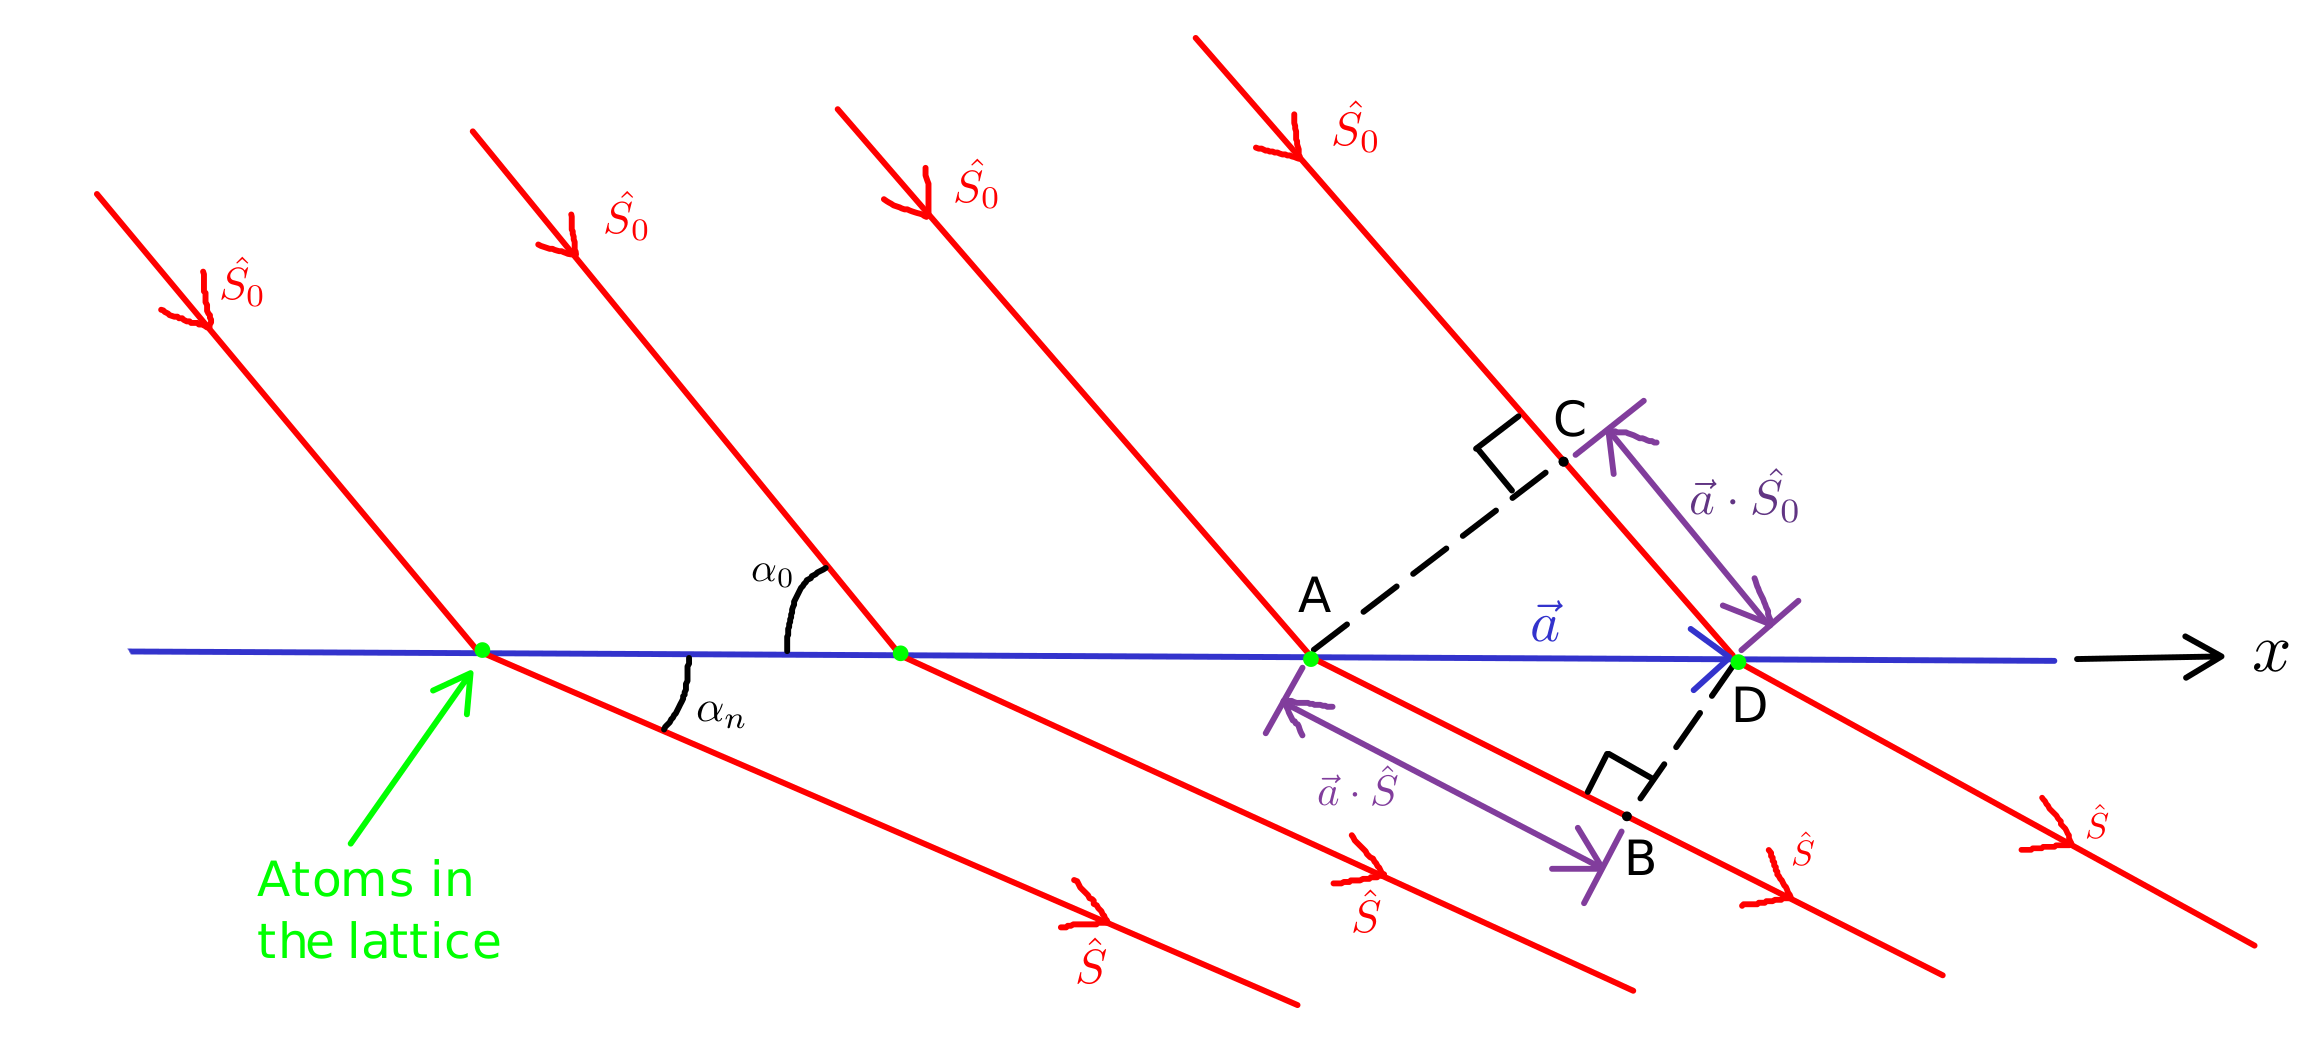
\includegraphics[scale=0.17]{laue_analysis.png}
	\caption{\label{fig:laue_analysis}Diffraction from a lattice row along the $x$ axis. The incident and diffracted beams make angles $\alpha_0$ and $\alpha_n$ respectively with the lattice row. $\vec{a}$ is the lattice translation vector. Adapted from \cite{Hammond2015}.}
	\end{figure}
	
	Consider a simple crystal with one atom as the basis, as shown in figure~\ref{fig:laue_analysis}. The atoms are regarded as the scattering centres from which the diffraction takes place. $\hat{S_0}$ and $\hat{S}$ are two unit vectors in the direction of the incident and diffracted beam, respectively. The lattice spacing is $a$.
	
	The path difference,%
%		
		\begin{align}
		\mathrm{P.D.} &= \mathrm{AB - CD}, \nonumber\\
					  &= a \qty( \cos \alpha_n - \cos \alpha_0 ) \\
					  &= \va{a} \cdot \qty( \vu{S} - \vu{S_0} ),
		\end{align}%
%		
	has to be an integer multiple of wavelength for constructive interference.%
%		
		\begin{equation}
		\therefore \boxed{a \qty( \cos \alpha_n - \cos \alpha_0 ) = \va{a} \cdot \qty( \vu{S} - \vu{S_0} ) = n_x \lambda,} \quad n_x \in \mathbb{Z}. \label{eq:1st_laue_eqn}
		\end{equation}
		
	Eqn.~\eqref{eq:1st_laue_eqn} is the \textbf{first Laue equation}.
	
	This path difference is still valid if the diffracted beam, instead of being below the row of atoms, is above it, or is out of the plane of the paper itself. Therefore, all diffracted beams with the same path difference occur at the same angle to the atom row. Thus, all diffracted beams lie on the surface of a cone, known as the \bfnt{Laue cone}, centred on the atom row with semi-apex angle $\alpha_n.$ This is illustrated in figure~\ref{fig:laue_cones}.
	
	\begin{figure}
	\centering
	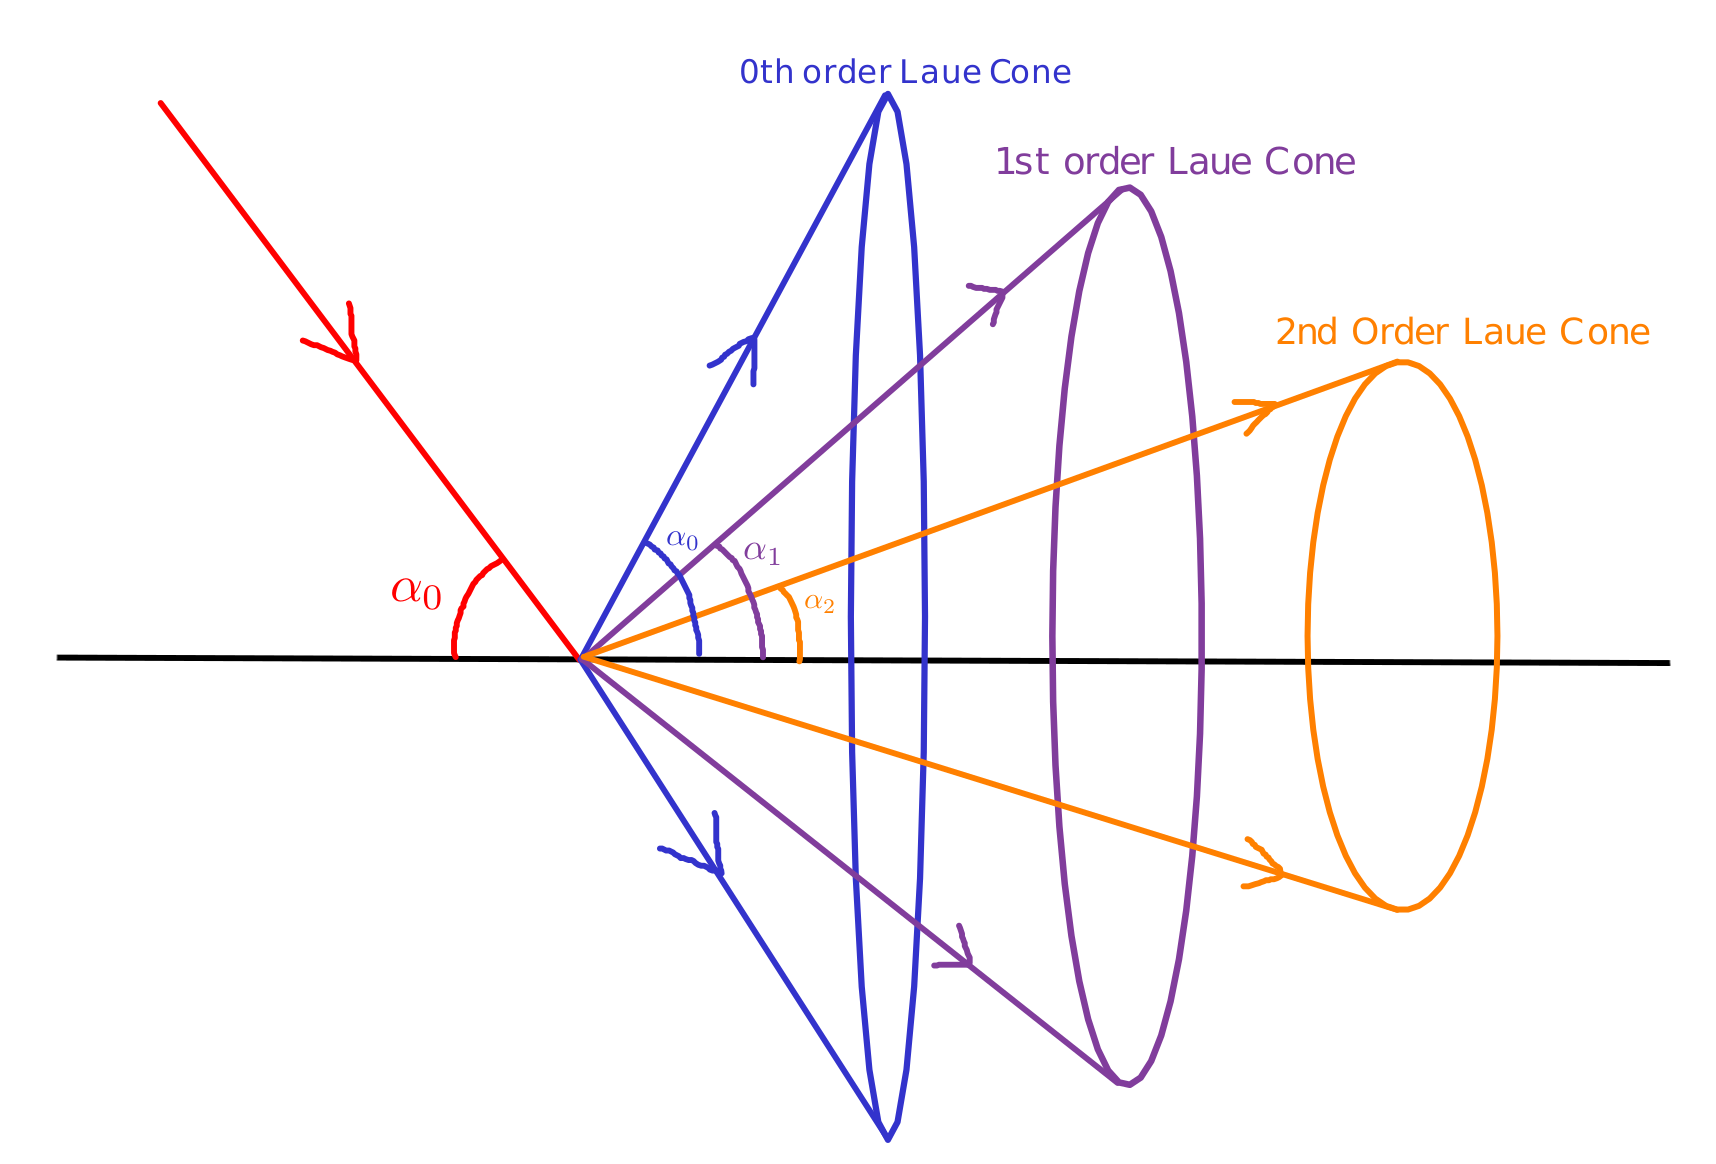
\includegraphics[scale=0.17]{laue_cones.png}
	\caption{\label{fig:laue_cones}Three Laue cones representing the direction of diffracted beam from a lattice row along the $x$-axis, with $0$ ($n_x = 0$), $\lambda$ ($n_x = 1$) and $2\lambda$ ($n_x = 2$) path differences. Similar cones also lie to the left of the 0th order cone for $n < 0.$}
	\end{figure}
	
	Proceeding similarly, we can derive two more equations for diffraction from atom rows along the $y$ and $z$ directions, thereby arriving at the second and third Laue equations:%
%		
	\begin{align}
	\boxed{b \qty( \cos \beta_n - \cos \beta_0 ) = \va{b} \cdot \qty( \vu{S} - \vu{S_0} ) = n_y \lambda,} \quad n_y \in \mathbb{Z}; \label{eq:2nd_laue_eqn} \\[1.5em]
	\boxed{c \qty( \cos \gamma_n - \cos \gamma_0 ) = \va{c} \cdot \qty( \vu{S} - \vu{S_0} ) = n_z \lambda,} \quad n_z \in \mathbb{Z}. \label{eq:3rd_laue_eqn}
	\end{align}
	
	For constructive interference to simultaneously occur from all the three atom rows in the three directions, all three Laue equations must be satisfied simultaneously. This is geometrically equivalent to three Laue cones intersecting at some points. Diffraction will only occur along those directions in which three Laue cones intersect.
	
%***********************************************************************************************


\subsection{The reciprocal lattice}

	\begin{figure}
	\centering
	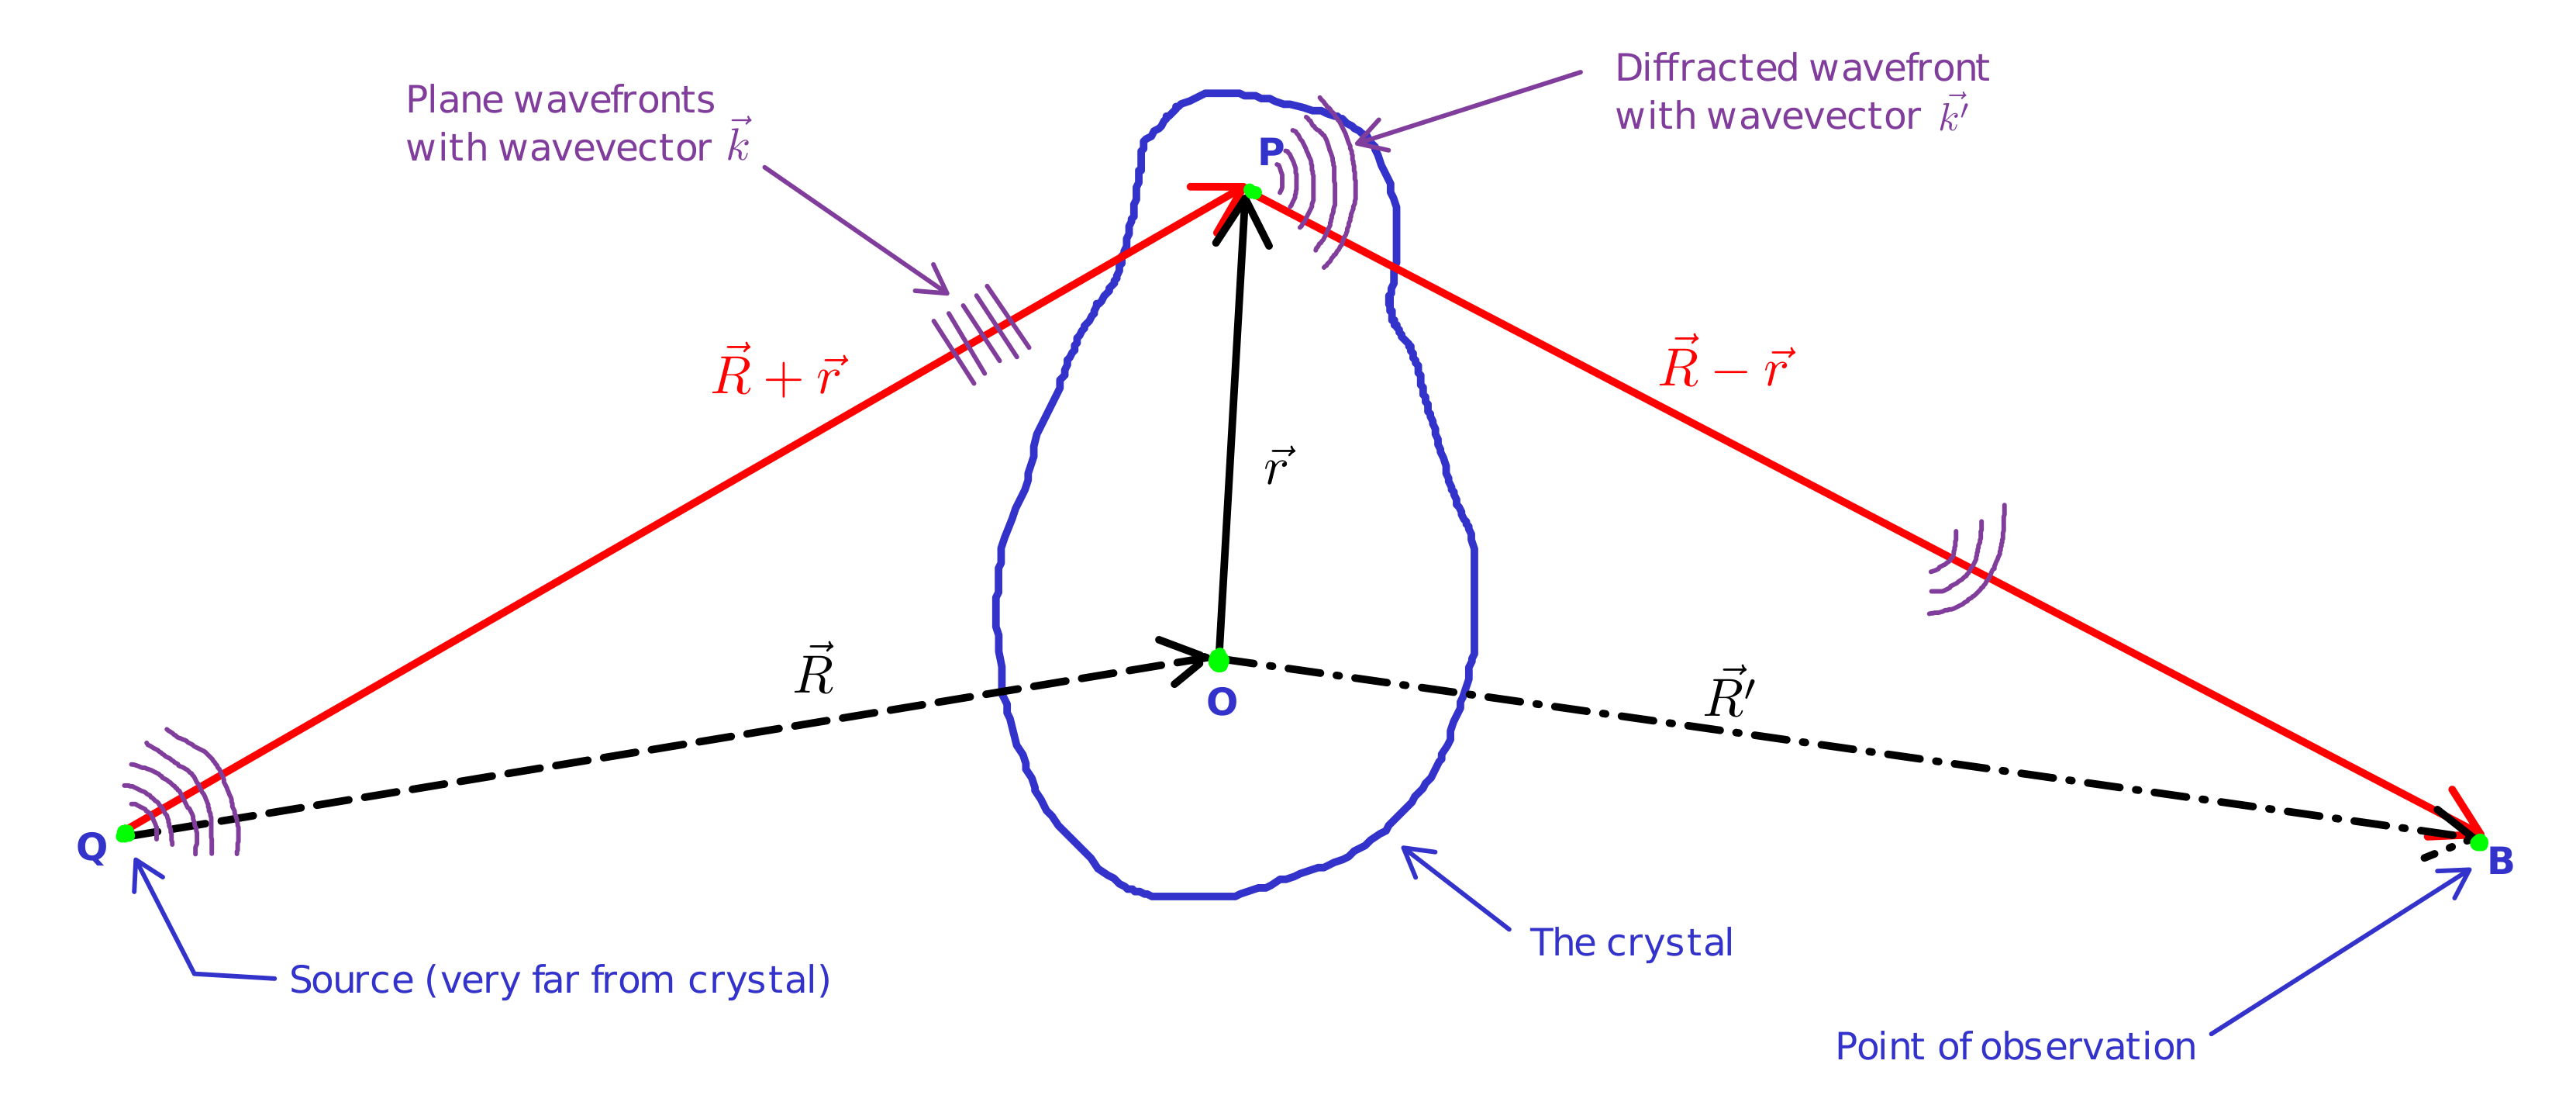
\includegraphics[width=\textwidth]{reciprocal_lattice.png}
	\caption{\label{fig:reciprocal_lattice}A plane wavefront with wavevector $\va{k}$ reaches a crystal, and is diffracted by an atom at point $P.$ We observe the diffracted beam, with wavevector $\va{k'}$, from point $B.$ Figure adapted from \cite{Harbola2021}.}
	\end{figure}

	Consider the situation shown in figure~\ref{fig:reciprocal_lattice}. The source of X-rays is very far away from the crystal; hence, the wavefront reaching the crystal can be considered to be a plane wavefront. We observe from point $B.$
	
	The plane wave reaches the point $P$ with an amplitude%
%		
		\begin{equation}
		A_P = A_0 ~ \e{i \va{k} \vdot \qty( \va{R} + \va{r} )} ~ \e{-i \omega_0 t}
		\end{equation}

	The amplitude of the waves reaching $B$ will depend on $A_P$ and density of scatterers at $P.$ The spherical waves generated from $P$ and reaching point $B$ will have the form%
%		
		\begin{equation}
		A_B = A_P ~ \rho(\va{r}) ~ \dfrac{\e{i \va{k'} \vdot ( \va{R'} - \va{r} ) }}{\abs{ \va{R'} - \va{r} }},
		\end{equation}%
%		
	where $\rho(\va{r})$ is the density of scatterers at $P.$ We assume that these scatterers are all in phase, and act as secondary sources.\\
	
	Assume $\va{R'} \gg \va{r}.$\\[0.8em]
	$\implies \abs{ \va{R'} - \va{r} } \approx \abs{\va{R'}} = R'$
	
	\begin{align}
	\therefore A_B &= \dfrac{A_0 \rho(\va{r})}{R'} ~ \e{i \va{k} \vdot ( \va{R} + \va{r} )} ~ \e{ i \va{k}' \vdot (  \va{R}' - \va{r}) } \nonumber \\[0.8em]
		&= \underbrace{\dfrac{A_0 \rho(\va{r})}{R'} ~ \e{ i ( \va{k} \vdot \va{R} + \va{k}' \vdot \va{R}' ) }}_{\text{constant}} ~ \e{i ( \va{k} - \va{k'} ) \vdot \va{r}}.
	\end{align}
	
	Let%
%		
		\begin{equation}
		\va{\kappa} = \va{k}' - \va{k}
		\end{equation}%
%		
	be the \textbf{scattering vector}.
	
	The net intensity due to all such points $P$ in the crystal is given by%
%		
		\begin{align}
		I &\propto \abs{ \int_V A_B(\va{r}) \dd[3]{r} }^2 \nonumber \\[1em]
		  &\propto \dfrac{A_0^2}{R'^2} \abs{ \int_V \dd[3]{r} \rho(\va{r}) ~ \e{ - i \va{\kappa} \vdot \va{r} } }  ^2. \label{eq:net_I}
		\end{align}
		
	$\va{R}$ is the lattice translation vector, defined by%
%		
	\begin{equation}
	\va{R} = \sum_{i=1}^3 n_i \va{a}_i
	\end{equation}%
%	
	where $\va{a}_i$ are the basis vectors, and $n_i \in \mathbb{Z} ~ \forall ~ i.$
	
	Expanding $\rho(\va{r})$ in terms of Fourier components,%
%		
	\begin{equation}
	\rho(\va{r}) = \sum_{\va{G}} \rho_{\va{G}} ~ \e{ i \va{G} \vdot \va{r} } \label{eq:fourier_rho}
	\end{equation}
%	
	and%
%	
	\begin{equation}
	\rho(\va{r} + \va{R}) = \sum_{\va{G}} \rho_{\va{G}} ~ \e{ i \va{G} \vdot \va{r} } ~ \e{ i \va{G} \vdot \va{R} }.
	\end{equation}
	
	Due to translational invariance in a Bravais lattice,%
%	
	\begin{align}
	&\phantom{\implies} \rho (\va{r}) = \rho( \va{r} + \va{R} ) \nonumber \\
	&\implies \boxed{ \e{i \va{G} \vdot \va{R} } = 1.} \\ \label{eq:reci_lattice_cond}
	&\implies \va{G} \vdot \va{R} = 2\pi m, \quad m \in \mathbb{Z}.
	\end{align}
	
	This $\va{G}$ is the translation vector of the reciprocal lattice. Given any lattice in real space, we can generate a lattice in reciprocal space keeping in mind equation~\eqref{eq:reci_lattice_cond}.
	
	If%
%	
	\begin{equation}
	\va{G} = h \va{g}_1 + k \va{g}_2 + \ell \va{g}_3,\label{eq:reci_lattice_vec}
	\end{equation}%
%	
	then we have%
%	
	\begin{equation}
	\va{g}_i \vdot \va{a}_j = 2\pi \delta_{ij}.\label{eq:relation_g_a}
	\end{equation}%
	
	One expression that satisfies this condition is%
%	
	\begin{equation}
	\va{g}_1 = 2\pi \dfrac{\va{a}_2 \cross \va{a}_3}{\qty[ \va{a}_1 ~ \va{a}_2 ~ \va{a}_3 ]}
	\end{equation}%
%	
	and so on.
	
	Returning to Eqn.~\eqref{eq:net_I}, substituting eqn.~\eqref{eq:fourier_rho}, we have%
%	
	\begin{align}
	I &\propto \dfrac{A_0^2}{R'^2} \abs{ \sum_{\va{G}} \int_V \dd[3]{r} \rho_{\va{G}} ~ \e{ i (\va{G} - \va{\kappa}) \vdot \va{r} } }  ^2 \nonumber \\[1em]
	  &\propto \dfrac{A_0^2}{R'^2} \abs{ \sum_{\va{G}} \rho_{\va{G}} \int_V \dd[3]{r} \e{ i (\va{G} - \va{\kappa}) \vdot \va{r} } }^2
	\end{align}%
	
	If $\va{G} = \va{\kappa},$ the above integral evaluates to $V.$ If $\va{G} \ne \va{\kappa},$ the integral is $0$ as it an integration of sines and cosines over the entire volume. Thus,%
%	
	\begin{equation}
	\int_V \dd[3]{r} \e{ i (\va{G} - \va{\kappa}) \vdot \va{r} } = \delta ( \va{G} - \va{\kappa} ) \cdot V.
	\end{equation}
	
	Therefore, the condition under which $I \ne 0$ is%
%	
	\begin{equation}
	\boxed{\va{\kappa} = \va{G}}
	\end{equation}%
%	
	i.e. when the reciprocal space lattice translation vector = scattering vector. This is known as \bfnt{Laue's condition} for X-ray diffraction.
	
	As a parting note, it should be mentioned that the vector $\va{G}_{hk\ell},$ written as in eqn.~\eqref{eq:reci_lattice_vec}, is perpendicular to the plane whose Miller indices are given by $(h k \ell).$
		
%--------------------------------------------------------------------------------------------------

\subsection{Ewald's Sphere}
	
	\begin{figure}
	\centering
	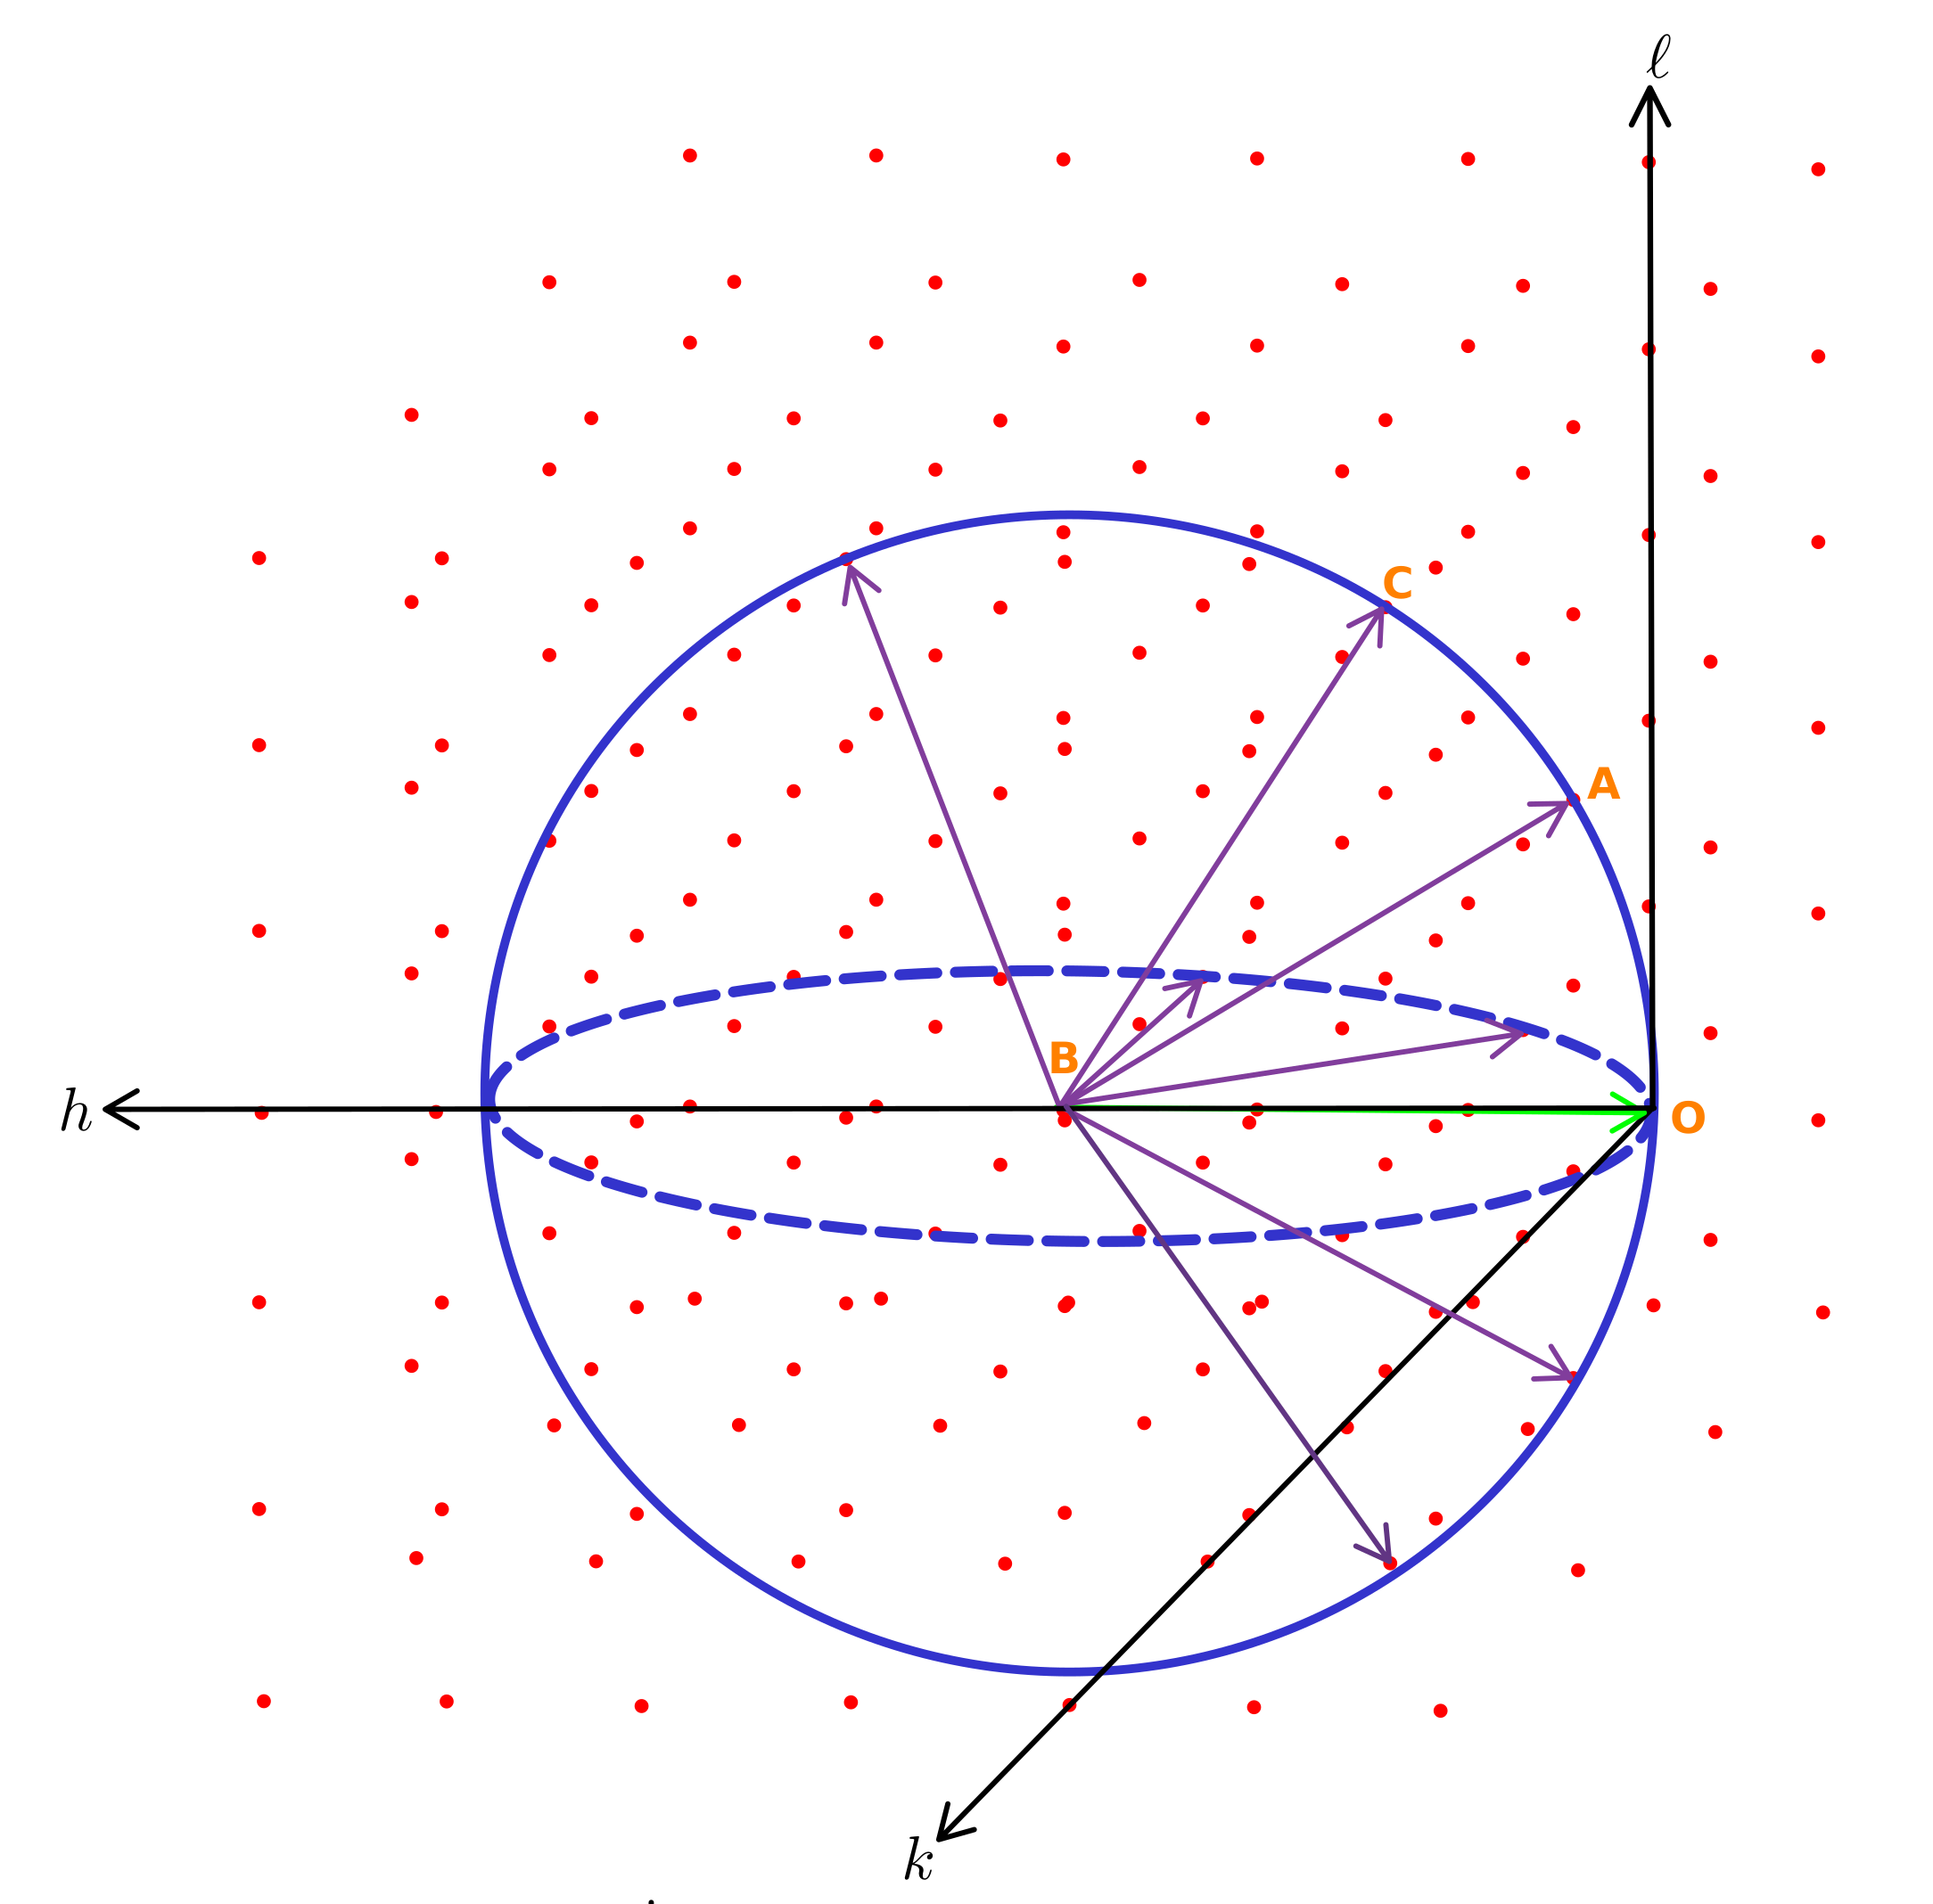
\includegraphics[scale=0.15]{ewald_sphere.png}
	\caption{\label{fig:ewald_sphere}Ewald's sphere construction in three dimensional reciprocal space. Each point in the reciprocal space corresponds to a set of planes in the real space with Miller indices same as that of the coordinates of the point. The green line is the wave vector of the incident X-ray beam, with $\overrightarrow{BO} \equiv \va{k}.$ We draw the sphere with the origin at the tail of the incident wave vector, $B,$ and with a radius~$= \abs*{\va{k}} = 2\pi / \lambda.$ The blue sphere thus drawn is Ewald's sphere. All the purple arrows are vectors which end on points on the surface of the sphere. These points satisfy Bragg's Law; therefore, the purple arrows are actually the wave vectors of the X-ray beam diffracted from that particular set of planes.}
	\end{figure}
	
	Refer to figure~\ref{fig:ewald_sphere}. In 3D reciprocal space, each point $(h, k, \ell)$ denotes a particular plane in real space with Miller indices $(hk\ell).$ The vector $\overrightarrow{BO} \equiv \va{k}$ is the wave vector of the incident X-ray beam. A sphere is drawn with the tail of the incident wave vector (point $B$) as the origin, and with a radius~$= \abs*{\va{k}} = \frac{2\pi}{\lambda}.$ This sphere, shown in blue, is Ewald's sphere or the reflecting sphere. Note that the tip of the arrow is taken as the origin of the coordinate system.
	
	In elastic scattering, the wave vector of the diffracted beam will have the same length as that of the incident wave vector, i.e. $\abs*{\va{k}'} = \abs*{\va{k}}.$  Therefore, \textcolor{red}{any point on the surface of the sphere will denote a set of planes that satisfy Bragg's Law}.
	
	Consider the point $A(h_1, k_1, \ell_1).$ It lies on the surface of the sphere, and hence, the set of planes with Miller indices $(h_1 k_1 \ell_1)$ will satisfy Bragg's Law. $\overrightarrow{BA}$ will be the wave vector of the diffracted beam, and $\angle ABO = 2\theta,$ where $\theta$ is the Bragg angle for this particular set of planes. The scattered wave vector $\va{\kappa}$ will be, in this case, $\overrightarrow{AO},$ and, due to Laue's condition, this is the same as the reciprocal lattice vector $\va{G}.$ Thus, we may visualize the incident beam hitting the crystal planes at the point $B,$ and the planes are oriented such that $AO$ is perpendicular to them.
	
	Ewald's sphere, thus, helps us to geometrically understand Laue's condition and the unification of Bragg's Law and Laue's condition.
	
%******************************************************************************************************

\subsection{Structure Factor, Friedel's Law and Centrosymmetry in X-ray Diffraction}

	The atomic scattering factor is given by%
%	
	\begin{equation}
	f = \dfrac{\text{Amplitude scattered by atom}}{\text{Amplitude scattered by single electron}}.
	\end{equation}
	
	At zero scattering angle, all the scattered waves are in phase and the scattered amplitude is the simple sum of the contribution from all $Z$ electrons, i.e. $f = Z$. As the scattering angle increases, $f$ falls below $Z$ because of the increasingly destructive interference effects between the $Z$ scattered waves.

	The scattering amplitude of a unit cell is determined by summing $f$ from all the atoms in a unit cell to all the atoms in a basis. The summation must take into account the path or phase differences between the scattered wave, and is given by the dimensionless structure factor:%
%	
	\begin{equation}
	F_{hk\ell} = \dfrac{\text{amplitude scattered by the atoms in the unit cell}}{\text{amplitude scattered by a single electron}}.
	\end{equation}
	
	$F_{hk\ell}$ must include the phase angle of the scattered wave, and hence, it is a complex number.
	
	\begin{figure}
	\centering
	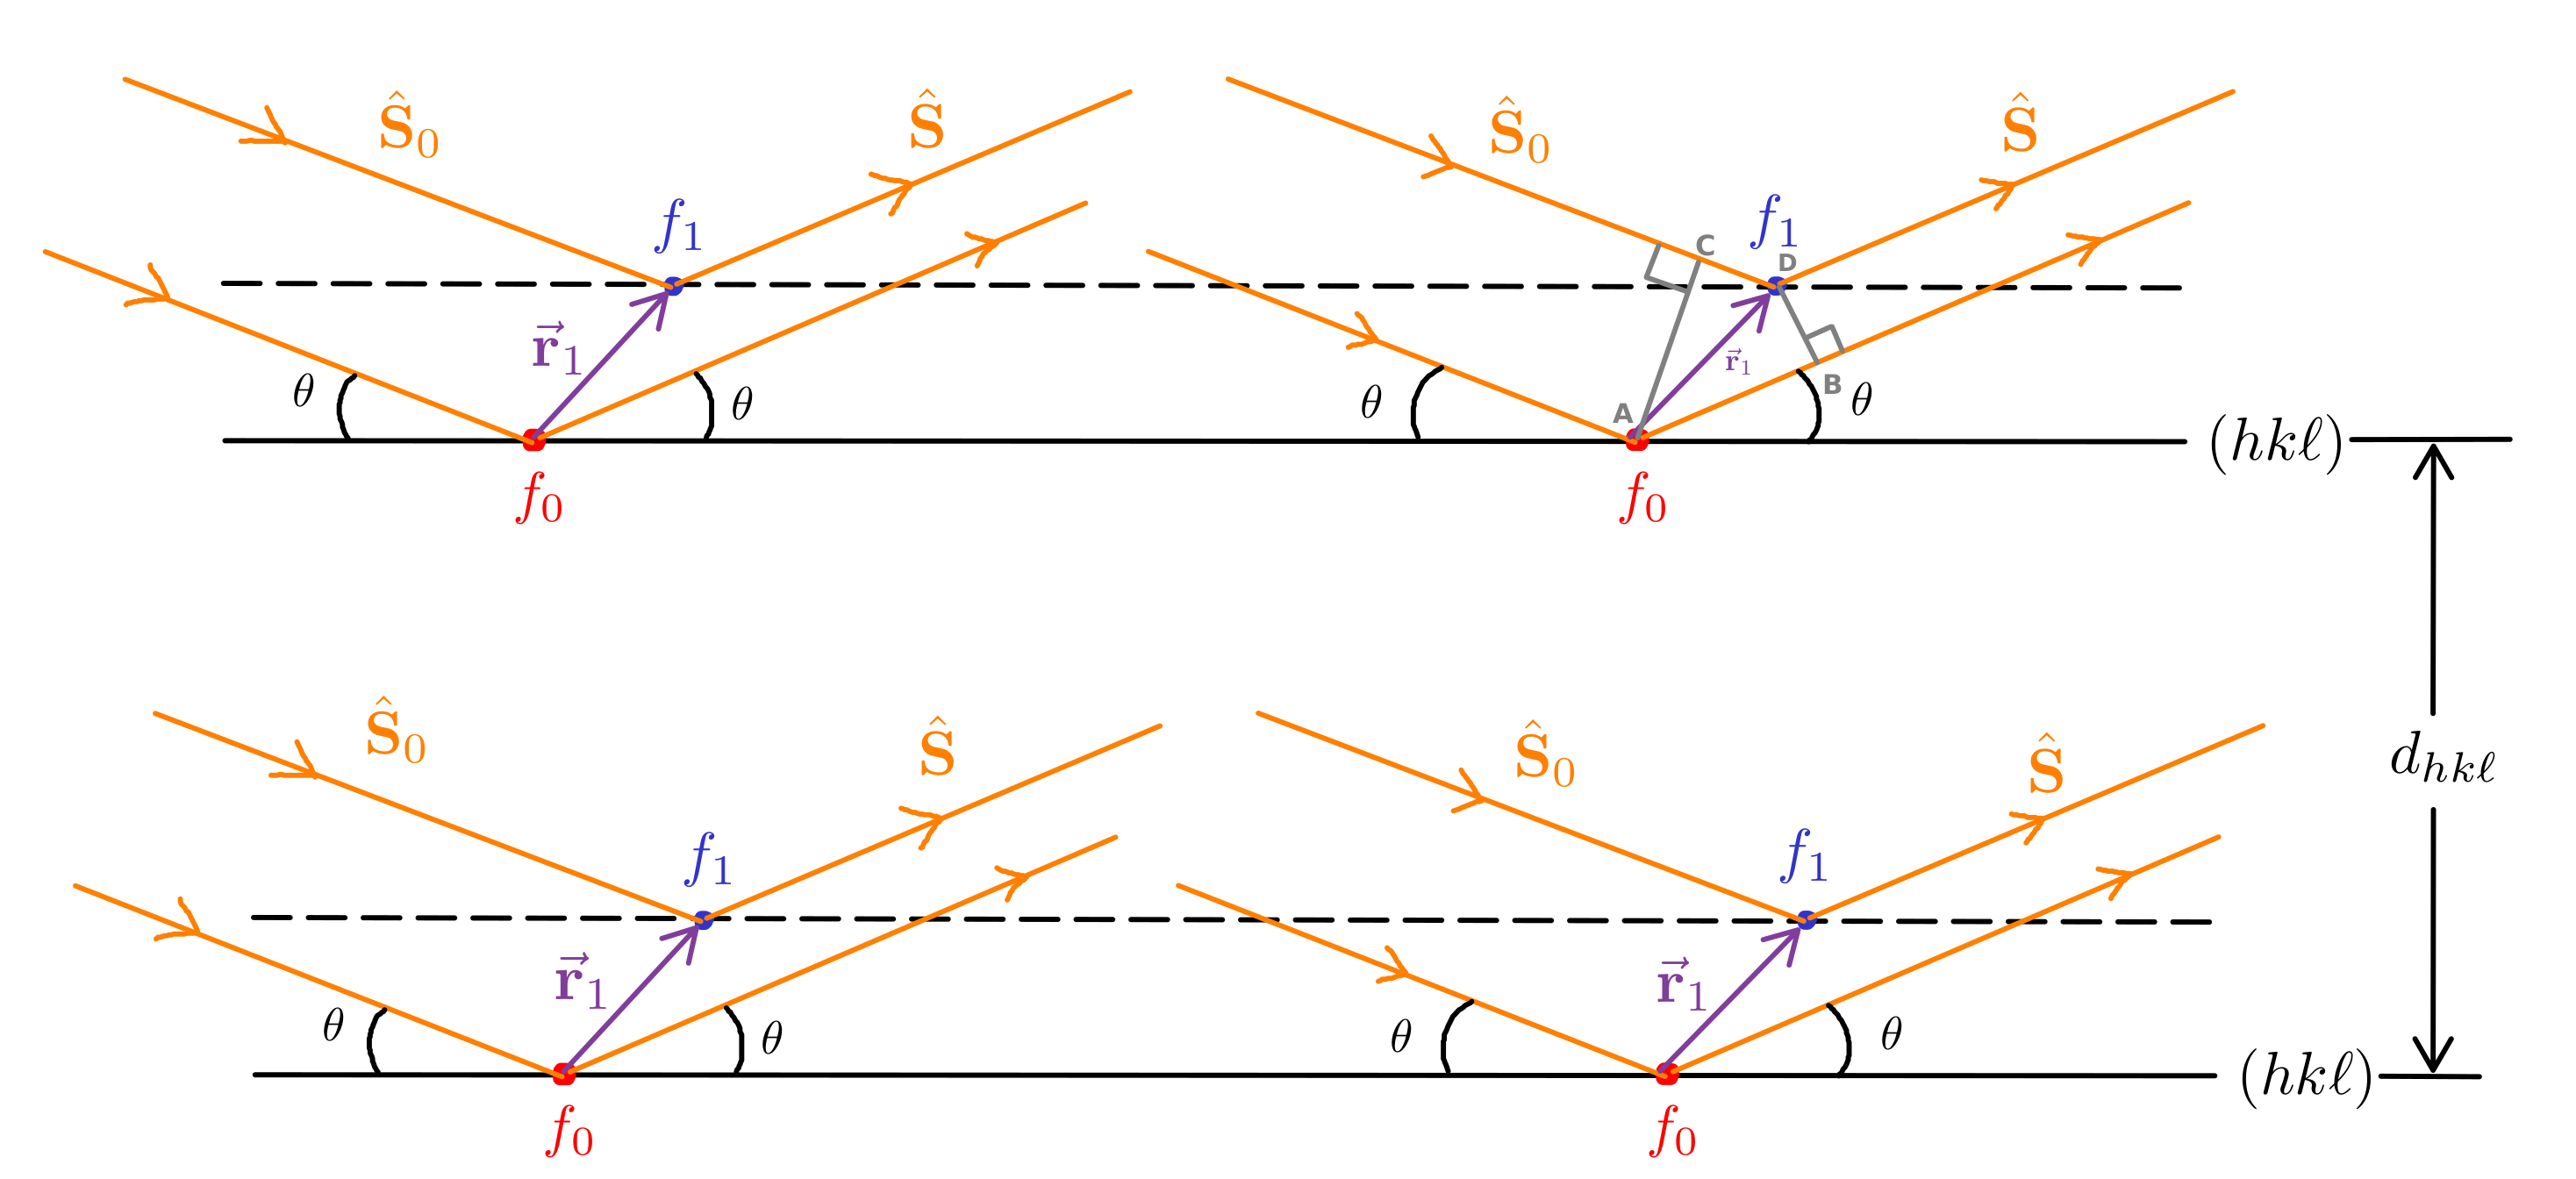
\includegraphics[scale=0.15]{structure_factor.png}
	\caption{\label{fig:struct_fact}Consider a basis with two atoms, one with atomic scattering factor $f_0$, and another with $f_1.$ $\va{r}_1$ is the position vector of one atom w.r.t. the other. $\vu{S}_0$ is a unit vector in the direction of the incoming X-ray beam, while $\vu{S}$ is the unit vector in the direction of the diffracted beam.}
	\end{figure}
	
	Refer to figure~\ref{fig:struct_fact}. The position vector $\va{r}_1$ is written as%
%	
	\begin{equation}
	\va{r}_1 = \sum_{i=1}^3 x_i \va{a}_i
	\end{equation}%
%	
	where $\va{a}_i$ are the lattice basis vectors, and $x_i$ are \textit{fractions} of the cell edge lengths.
	
	The path difference,%
%	
	\begin{align}
	\mathrm{P.D.} &= \mathrm{AB} - \mathrm{CD} \nonumber \\
				  &= \va{r}_1 \vdot \vu{S} - \va{r}_1 \vdot \vu{S}_0 \nonumber \\
				  &= \va{r}_1 \vdot ( \vu{S} - \vu{S}_0 ).
	\end{align}
	
	$\because$ Bragg's Law is satisfied, we can write using eqn.~XXX,%
%		
	\begin{align}
	&\phantom{\implies} ( \vu{S} - \vu{S}_0 ) = \lambda \va{G}_{hk\ell} \nonumber\\
	&\phantom{ \implies ( \vu{S} - \vu{S}_0 ) } = \lambda \qty( h \va{g}_1 + k \va{g}_2 + \ell \va{g}_3 ).\\
	&\implies \mathrm{P.D.} = \lambda \qty( x_1 \va{a}_1 + x_2 \va{a}_2 + x_3 \va{a}_3 ) \vdot \qty( h \va{g}_1 + k \va{g}_2 + \ell \va{g}_3 ) \nonumber \\
	&\implies \mathrm{P.D.} = \lambda \qty( h x_1 + k x_2 + \ell x_3 ).
	\end{align}%
%	
	where we have used $\va{g}_i \vdot \va{a}_j = \delta_{ij}$ to arrive at the last step.
	
	The phase angle is given by%
%	
	\begin{align}
	\phi &= \dfrac{2\pi}{\lambda} \mathrm{P.D.} \nonumber \\
		 &= 2 \pi \lambda \qty( h x_1 + k x_2 + \ell x_3 ).
	\end{align}
	
	There are two ways to add scattering amplitudes $f$ with their respective phase angles $\phi$ to arrive at the structure factor: by a vector space diagram, or in the Argand plane. We shall use the latter:%
%	
	\begin{equation}
	\boxed{F_{hk\ell} = \sum_{n = 1}^N f_n ~ \exp \qty[ 2\pi i \qty( h x_n + k y_n + \ell z_n ) ].}
	\end{equation}
	
	Consider the case of a crystal with a centre of inversion symmetry at the origin. For every atom with fractional coordinates $(x,y,z)$ and phase angle $+\phi,$ there will be an identical atom on the opposite side of the origin with fractional coordinates $(\bar{x}, \bar{y}, \bar{z})$ with phase angle $-\phi.$ Therefore,%
%	
	\begin{align}
	F_{hk\ell} &= f \exp \qty[ 2\pi i \qty( h x + k y + \ell z ) ] + f \exp \qty[ 2\pi i \qty( h \bar{x} + k \bar{y} + \ell \bar{z} ) ] \nonumber \\
		&= f \exp \qty[ 2\pi i \qty( h x + k y + \ell z ) ] + f \exp \qty[ - 2\pi i \qty( h x + k y + \ell z ) ] \nonumber \\
		&= 2f \cos 2\pi \qty( h x + k y + \ell z ).
	\end{align}%
	
	The intensity of the diffracted beam is given by%
%	
	\begin{align}
	I &\propto \abs{F_{hk\ell}} ^2 \nonumber \\
	  & \propto F_{hk\ell} \cdot F^*_{hk\ell}.
	\end{align}%
%	
	Therefore, for a centrosymmetric crystal, the diffraction pattern is also centrosymmetric.
	
	It can, in fact, be shown that except in the case of anomalous scattering, \textcolor{red}{even if a crystal is not centrosymmetric (i.e. does not possess a centre of inversion symmetry), the diffraction pattern will still always be centrosymmetric}. This is known as \bfnt{Friedel's Law} and is mathematically written as%
%	
	\begin{equation}
	\boxed{I_{hk\ell} = I_{\bar{h} \bar{k} \bar{\ell}}.} \label{eq:friedel_law}
	\end{equation}
	
	The presence of a centre of symmetry in the diffraction pattern means that non- centrosymmetric crystals cannot be distinguished from those with a centre of symmetry. There are eleven centrosymmetric point groups and hence, eleven symmetries which \\diffraction patterns can possess. These are called the eleven \bfnt{Laue groups}. Only Laue groups can be distinguished from a X-ray diffraction pattern. Thus, the phase information in the structure factor is lost when we measure intensity of the diffracted beam.

%******************************************************************************************************

\subsection{Systematic absences}

	In X-ray diffraction experiments, the intensities of reflections from certain planes are zero. Such reflections are said to be \ifnt{systematically absent} since they arise from the centring of the unit cell and/or the presence of translational symmetry elements -- glide planes and screw axes.
	
	Systematic absence conditions can be derived in two ways: 1. through the geometrical consequences of using a centred, rather than a primitive, unit cell, and the presence of glides and screw axes, or 2. through the structure factor equation. The former is the proper approach as systematic absences arise solely from the architecture of the crystals.
	
	\begin{figure}
	\centering
	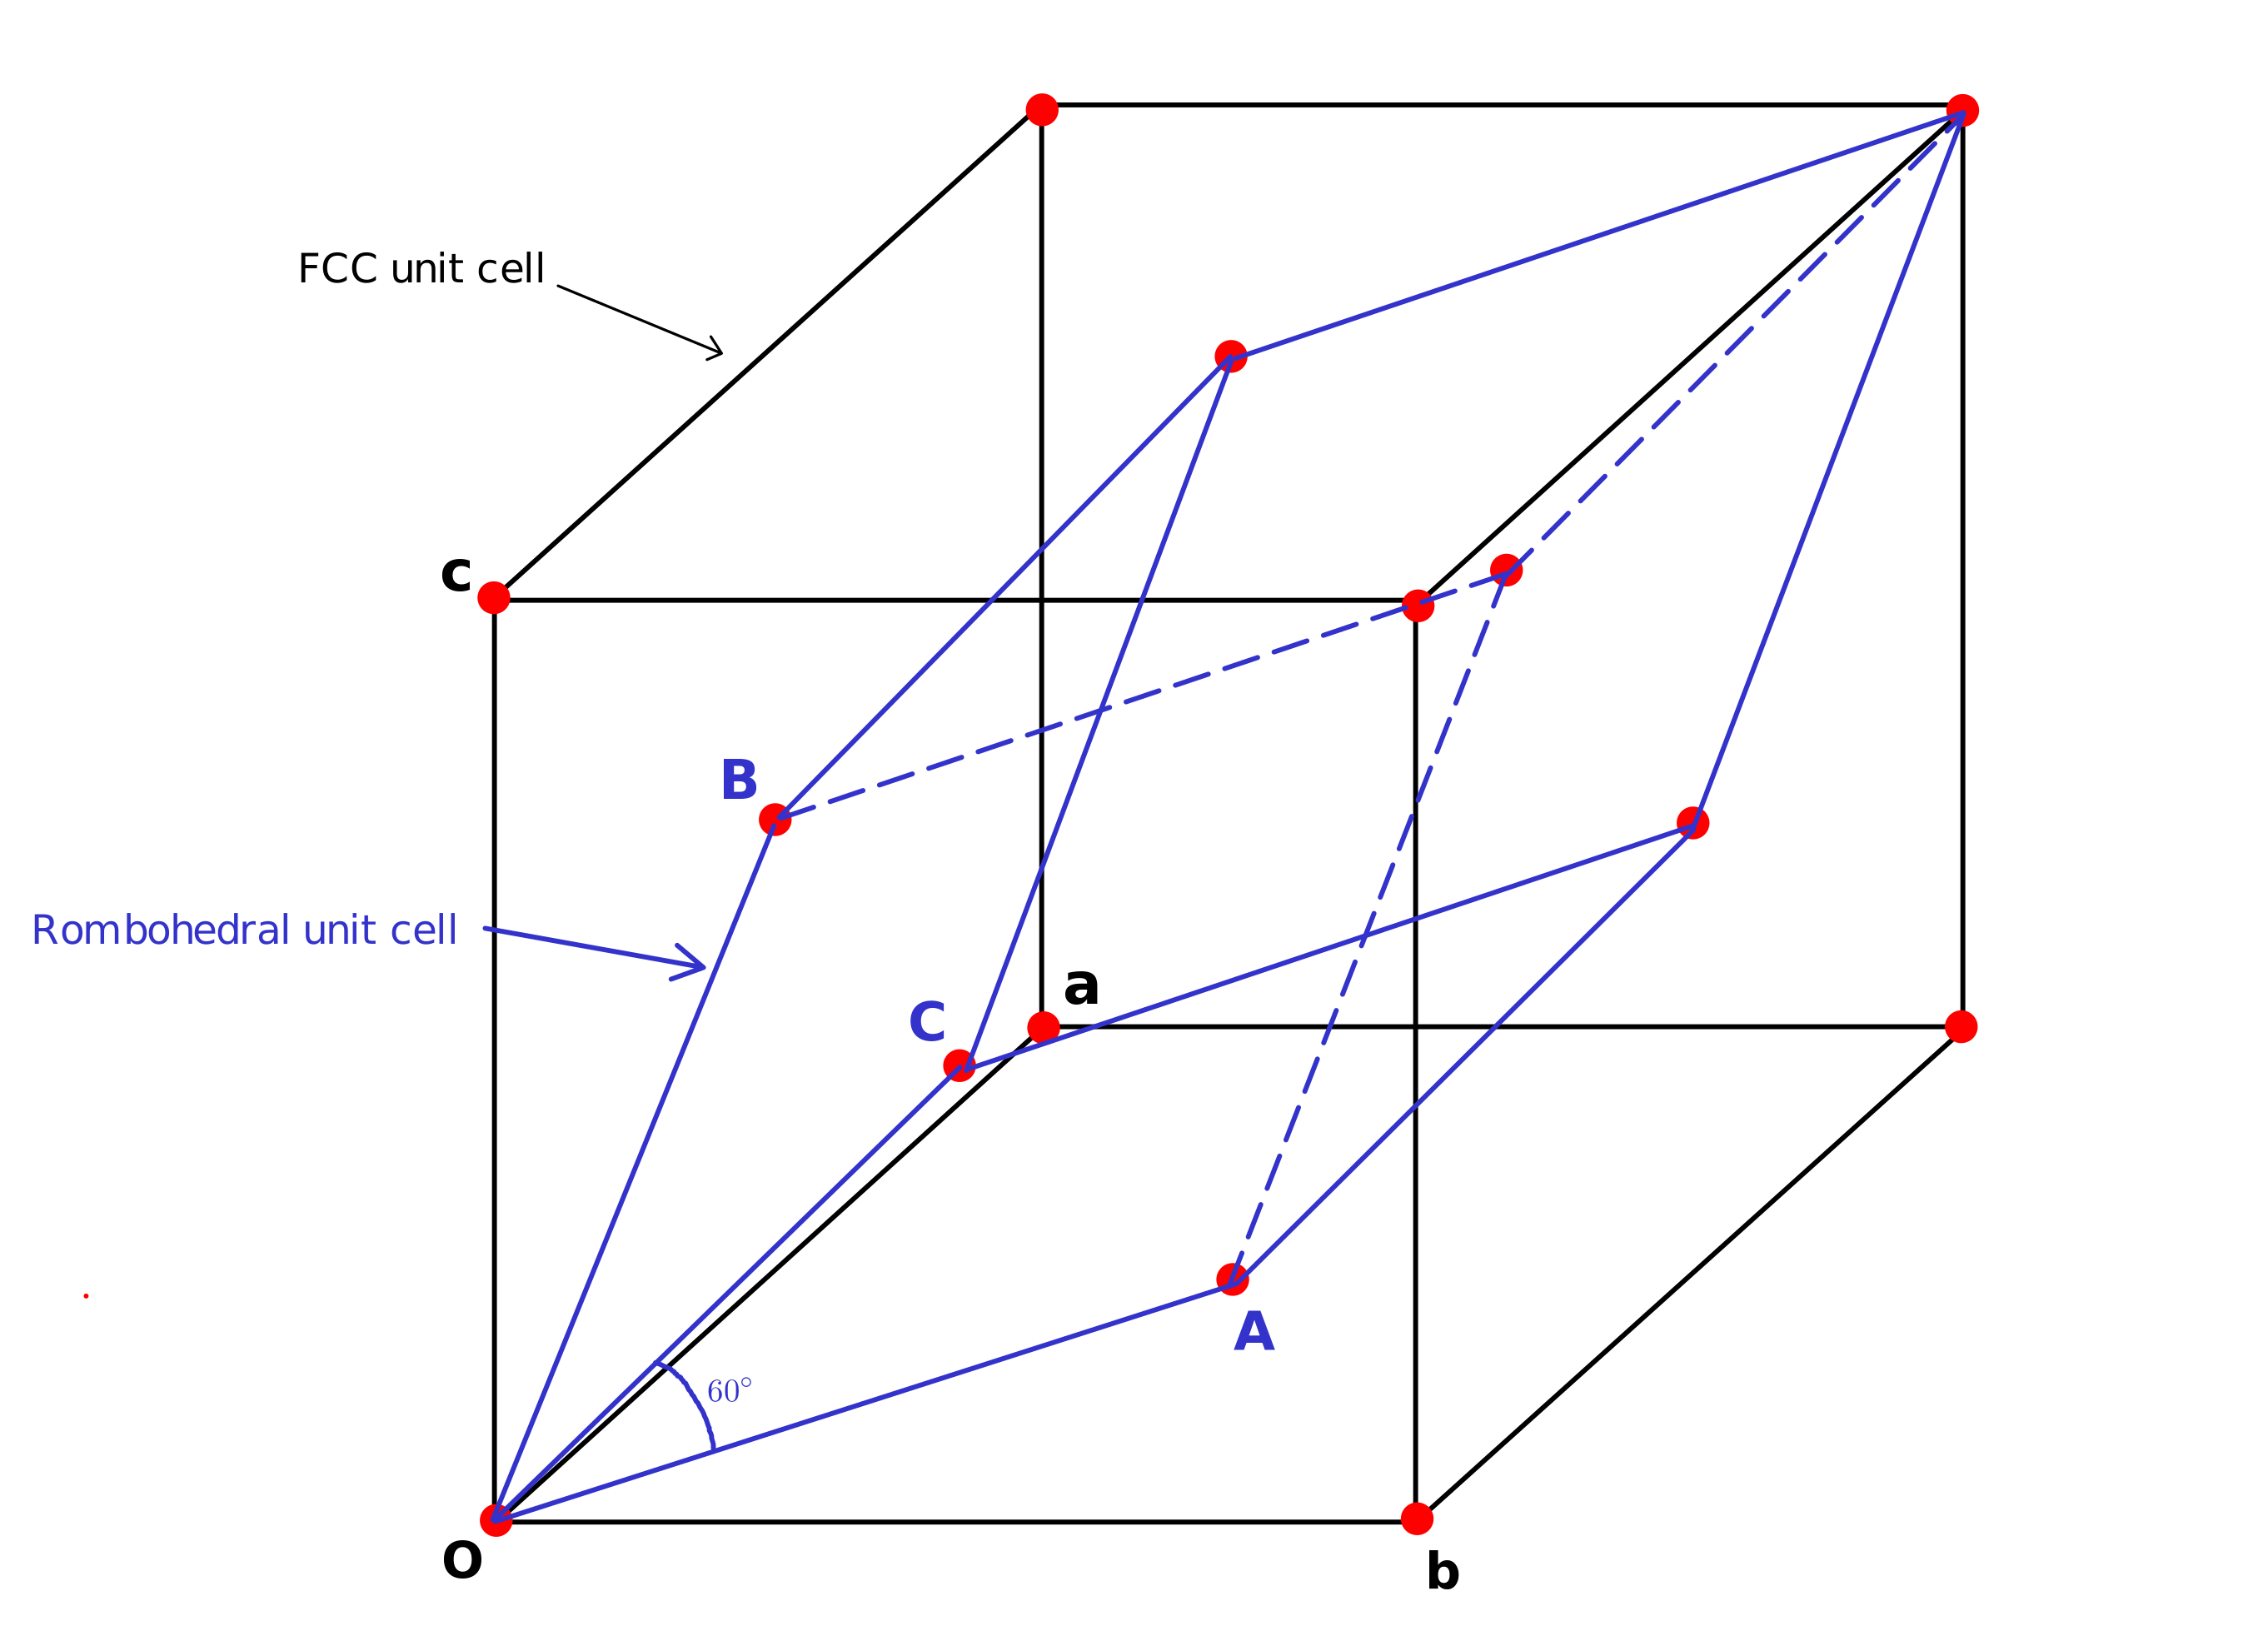
\includegraphics[scale=0.15]{fcc_lattice.png}
	\caption{\label{fig:fcc_fr}Cubic lattice with conventional face-centred unit cell, and a primitive rhombohedral unit cell.}
	\end{figure}
	
	Consider the cubic lattice shown in figure~\ref{fig:fcc_fr} with face-centred and rhombohedral unit cells. $\va{a}, \va{b}$ and $\va{c}$ are the basis vectors of the conventional FCC lattice, while $\va{A}, \va{B}$ and $\va{C}$ are the basis vectors of the primitive rhombohedral unit cell. The transformation equations are%
%		
	\begin{subequations}%
		\begin{align}
		\va{A} &= \frac{1}{2}\va{a} + \frac{1}{2}\va{b} + 0\va{c},\\[0.8em]
		\va{B} &= \frac{1}{2}\va{a} + 0\va{b} + \frac{1}{2}\va{c},\\[0.8em]
		\va{C} &= 0\va{a} + \frac{1}{2}\va{b} + \frac{1}{2}\va{c}.
		\end{align}
	\end{subequations}
	
	Miller indices follow the same transformation rules as unit cell vectors. Therefore,%
%	
	\begin{subequations}%
		\begin{align}
		H &= \frac{1}{2}h + \frac{1}{2}k + 0\ell \quad \implies 2H = h + k,\\[0.8em]
		K &= \frac{1}{2}h + 0k + \frac{1}{2}\ell, \quad \implies 2K = h + \ell,\\[0.8em]
		L &= 0h + \frac{1}{2}k + \frac{1}{2}\ell \quad \implies 2L = k + \ell.
		\end{align}
	\end{subequations}
	
	$\because H,K,L \in \mathbb{Z},$  $2H,\ 2K$ and $2L$ are all even integers, $\implies$ $h + k,\ h + \ell,$ and $k + \ell$ are also even integers.
	
	An even integer is the sum of either all odd or all even integers. Thus, reflections only occur from those lattice planes which have Miller indices $(hk\ell)$ all even or all odd. Planes for which the Miller indices are a mixture of off and even integers will be systematically absent in the X-ray diffraction peaks.
	
	Similar result can be derived using the structure factor equation, for body-centred cubic lattice, glide planes and screw axes.
	
%*********************************************************************************************

\subsection{Broadening of diffracted beams: the Scherrer equation}
	
	Till now, we have studied X-ray diffraction from a geometrical point of view. Incident and reflected beams were represented as perfectly collimated and narrow beams, and reflections occurred only at Bragg angles. This ideal situation is, in no way, the same as the practical situation as X-ray beams have a finite width and may not be perfectly parallel. Broadening of X-ray beams arise due to these instrumental factors. But, more importantly, inevitable line broadening arises from the crystallite size, perfection and state of strain of the specimen. The measurement of such broadening, after accounting for the instrumental factors, can give vital information about the specimen.
	
	The Scherrer equation is derived by considering a crystal of finite thickness $t$ $\perp$ the planes of interest, such that $m d_{h k \ell} = t.$ Next, we consider interference conditions for incident and reflected beams that are slightly deviated, say by $\delta \theta,$ from the Bragg angle. As we go to higher order reflections, or equivalently, planes with larger Laue indices, the path difference due to this deviated angle adds up to finally result in a destructive interference. The condition for destructive interference for the whole crystal is obtained by pairing up the higher order reflections, and after some approximations, we arrive at the Scherrer equation:%
%		
	\begin{equation}
	\beta = \dfrac{K \lambda}{t \cos \theta}
	\end{equation}%
%	
	where $\beta$ is the full width of the Bragg peak at half the maxima (FWHM), and $K$ is often referred \cite{Klug1974} to as the crystallite shape factor. $K$ depends \cite{Holzwarth2011} on the crystallite shape, the definitions of average crystallite size and width. The structure of Scherrer equation is not affected by these, but the numerical value of $K$ can change appreciably. In the absence of detailed information about the shape of the crystal, $K = 0.9$ is a good approximation.
	
	The Scherrer equation becomes particularly useful when studying nanostructures because peak broadening becomes significant \cite{AkankshaUrade2023} when the crystallite size drops to $50-25~\si{nm}.$ At around $\SI{10}{nm},$ peak intensities become weak, and peak broadening becomes significant as peaks often overlap with each other, making it difficult to index and analyze the data.